\subsubsection{Модуль формирования и отправки приглашений}
В административной панели университета реализован модуль, который позволяет формировать и отправлять приглашения как для преподавателей, так и для студентов. Этот модуль работает по следующему сценарию:

\begin{enumerate}
    \item При инициации приглашения администратор вводит адрес электронной почты и идентификатор кафедры (для преподавателя) или адрес электронной почты и идентификатор группы (для студента), после чего нажимает кнопку «Сформировать ссылку».

    \item Затем пользовательский интерфейс отправляет запрос на создание приглашения на сервер. Сервер проверяет права администратора, корректность введённых данных, генерирует уникальную ссылку приглашения и возвращает её обратно в интерфейс.

    \item В ответ пользовательский интерфейс получает от сервера объект с полем \textit{invite\_link} (ссылка приглашения), отображает администратору полученную ссылку, которую можно скопировать и отправить по электронной почте.
\end{enumerate}

На рисунке~\ref{fig:admin-invite} приведена последовательная диаграмма, иллюстрирующая полный процесс формирования и отправки приглашений: в верхней части~--- сценарий для преподавателя, в нижней части~--- сценарий для студента.

\begin{figure}[h]
    \centering
    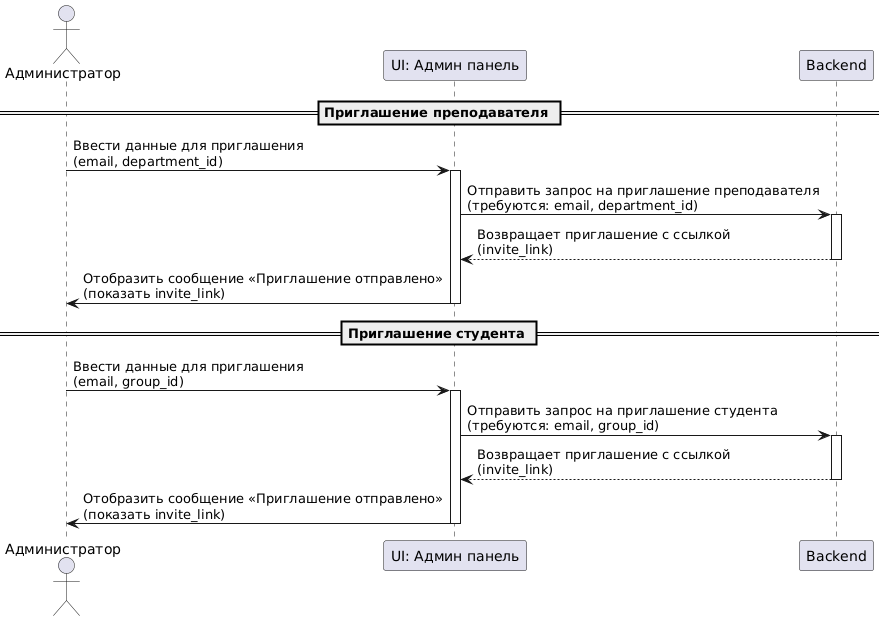
\includegraphics[width=0.9\textwidth]{static/diagrams/Admin.png}
    \caption{Схема процесса формирования и отправки приглашений преподавателям и студентам}
    \label{fig:admin-invite}
\end{figure}

На рисунке~\ref{fig:admin-invite} можно выделить следующие этапы:
\begin{enumerate}
    \item При приглашении преподавателя администратор вводит электронную почту и идентификационный номер кафедры. Пользовательский интерфейс отправляет запрос на сервер с указанными данными. Сервер проверяет данные, создаёт приглашение и возвращает уникальную ссылку. Пользовательский интерфейс отображает созданную ссылку.

    \item При приглашении студента администратор вводит электронную почту и идентификационный номер группы. Пользовательский интерфейс отправляет запрос на сервер с указанными данными. Сервер проверяет данные, создаёт приглашение и возвращает уникальную ссылку. Пользовательский интерфейс отображает созданную ссылку.
\end{enumerate}

Таким образом, схема на рисунке~\ref{fig:admin-invite} демонстрирует алгоритм работы модуля: ввод данных в пользовательский интерфейс, отправка запроса на сервер, генерация и возврат уникальной ссылки, отображение ссылки администратору.
